%=======================================================================
% Copyright (c) 2013 The University of York and Willink Transformations.
%
% $Id: icmt13_52.tex 4506 2013-02-12 16:45:23Z hhoyos@CS.YORK.AC.UK $
%=======================================================================
\documentclass{llncs}
%
\usepackage{makeidx}  % allows for indexgeneration
\usepackage{listings}
\usepackage{graphicx}
\usepackage{multicol}
%\usepackage{upquote}

%
\begin{document}
\lstset{
basicstyle=\scriptsize,
tabsize=4,
% Numbering
numbers=left, numberstyle=\tiny, numbersep=5pt}

\mainmatter              % start of the contributions
%
\title{Yet Another Three QVT  Languages}
%
\author{Edward Willink\inst{1} \and Horacio Hoyos\inst{2} \and Dimitris Kolovos\inst{2}}
%
\institute{Willink Transformations Ltd., Reading, UK \\
\email{ed@willinktransformations.co.uk}
\and The University of York, York, UK,\\
\email{horacio.hoyos.rodriguez@ieee.org, dimitris.kolovos@york.ac.uk},\\
}

\maketitle              % typeset the title of the contribution

%\begin{abstract}
The early enthusiasm, in 2002, for model to model transformation languages led to eight submissions for an OMG standard\cite{QVT1.1} comprising three languages, yet no commercial products. The QVT Core language was intended as the foundation for QVT Relations but the available implementations have ignored the core language. Rather than ignoring the core language, we take the opposite approach and introduce three more core languages. Progressive program-to-program transformation through these core languages terminates in an easily implemented imperative language that supports declarative transformations.

%\keywords{QVT, OCL, virtual machine, program transformation, declarative transformation, progressive transformation, transformation chain}
%\end{abstract}

%\section{Extended Abstract}
There are currently only two freely available but discouragingly stable implementations of QVTr. There are no implementations for QVTc. The Eclipse QVT Declarative project provides only models, editors and parsers for both QVTr and QVTc. We outline progress to remedy the execution deficiency.

The original work for  Eclipse QVTd execution considered only QVTr and confirmed that direct tooling of a complex declarative language such as QVTr is rather hard. Three years ago, the direct approach was abandoned and the progressive approach shown in the Figure was first posted on the web. Work on this approach has at last started.

\begin{figure}[h]
	\centering
	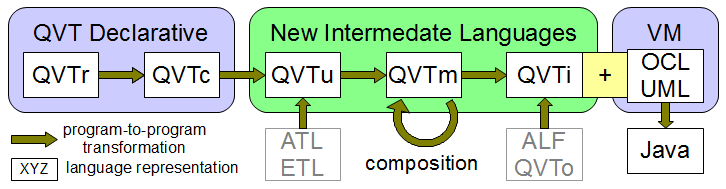
\includegraphics[width=0.9\textwidth]{QVThorizontalAlphabet.png}
%	\caption{Progressive transformation approach to Declarative QVT.}
	\label{fig:overview}
\end{figure}

At the left we have the two QVT Declarative languages, with QVTr realized by a QVTr to QVTc program-to-program transformation. Our three new languages, QVTu, QVTm and QVTi are syntactic and semantic simplifications of QVTc. QVTi is realized by extending the OCL support of Eclipse OCL. This enables the Xtext editing, OCL and UML model support and the OCL to Java code generator to be exploited.

The utility of the new languages and the program to program transformations are summarized below.

\subsubsection{QVTc to QVTu (Unidirectional)}
The QVTc transformation is aligned to the user's invocation context to extract a uni-directional declarative representation.
\begin{itemize}
\item the redundant multi-directionality and enforcement modes are eliminated
\end{itemize}

\subsubsection{QVTu to QVTm (Minimal)}
The QVTu transformation is normalized to give as simple and as uniform a declarative representation as possible.
\begin{itemize}
\item syntactic sugar is removed
\item representation alternatives are normalized
\end{itemize}

\subsubsection{QVTm to QVTi (Imperative)}
A practical multi-pass implementation is synthesized that can be easily executed on a model-friendly Virtual Machine.
\begin{itemize}
\item a reconciler is synthesized if an update transformation is required
\item a pattern matching schedule serializes declarative input matches
\item a pattern generation schedule serializes declarative output updates 
\end{itemize}

QVTc differs from other transformation languages in requiring traceability to be made explicit in an additional middle metamodel. QVTi exploits the middle model to provide a convenient buffer between the reconciliation, input matching and output update passes. The reconciliation for an update transformation populates the middle model with the pre-existing matches. An in-place transformation ensures that all input context is cached in the middle model before any potentially conflicting output updates are made. A solution to these complexities is prepared at compile time, and expressed in QVTi, so that the run-time execution is naive and efficient.  

These new languages are not just a convenience for realizing QVTc, they also offer important interchange points for other transformation technologies to exploit and so share the tool chain.

\begin{itemize}
\item QVTu provides a high level interchange point for other uni-directional declarative transformation languages such as ATL or ETL.
\item QVTm provides a normalized representation at which declarative transformation composition and optimisation can be applied.
\item QVTi provides a low level interchange point that imperative transformation languages such as QVTo, ALF or EOL may exploit.
\end{itemize}

The extension of Eclipse OCL VM\cite{Willink2012} to support execution of QVTi proved to be surprisingly easy. Some simple transformations have confirmed how simple QVTi  can be. It is now only necessary to develop the QVTr to QVTc to QVTu to QVTm to QVTi program transformation chain.
\bibliographystyle{splncs03}
\bibliography{hhr502References}
\end{document}